\documentclass[../main.tex]{subfiles}

\begin{document}

\problem{3}

One-dimensional, steady, compressible flow is used for a number of real-world applications, including: normal shock waves, bow shock waves, etc.
Look up some images or videos of normal shock waves and bow shock waves in front of bullets, re-rentry vehicles, etc. 
A schematic illustrating such flow is given below, where the flow entering the dashed control volume is given as state 1 and the flow exiting as state 2.
We will learn later in the semester that these properties do indeed change across shock waves.
For now, we will focus on simplifying our governing equations for these assumptions. 

\begin{figure}[ht]
    \centering
    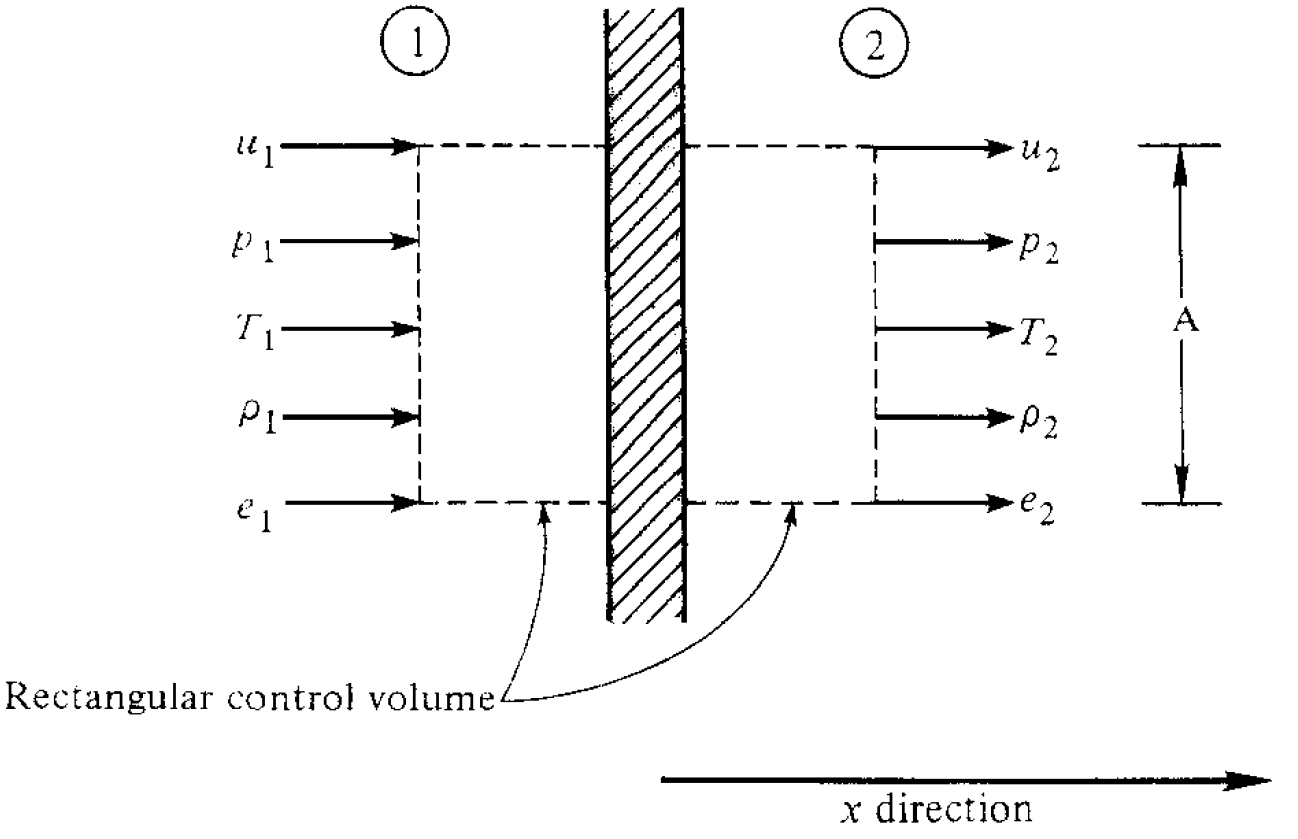
\includegraphics[scale=0.5]{images/problem3_diagram.png}
\end{figure}

In our one-dimensional, steady analyses, we will make the following assumptions about our flow:

\begin{enumerate}[label = (\roman*)]

    \item One-dimensional in the $x$ direction
    \item Steady
    \item Uniform velocity, pressure, temperature, density, enthalpy, and energy at each of the two control surfaces
    \item Flow is perpendicular to control surfaces 1 and 2
    \item \(A_1 = A_2\)
    \item No body forces present
    \item No friction/shear (i.e., there are no solid boundaries around)
    \item No work is done
    \item The pressures acting on the control volume in the $y$ and $z$ directions apply no net force

\end{enumerate}

\begin{enumerate}[label = (\alph*)]

    \item 
        Under these assumptions for one-dimensional, steady flow, show that the integral form of the continuity equation simplifies to
        \[
            \rho_1 u_1 = \rho_2 u_2 \, .  
        \]
        You must start with the full integral form and indicate which assumption(s) allowed you to make each simplification.
   
        The full form of the continuity equation is given by:

        \begin{equation*}
            \frac{\dd (m)_{sys}}{\dd t} = %
            \pdv{t} \int_{CV} \rho \dd \volume +%
            \int_{CS} \rho \left({\vec{V} \cdot \hat{\mathbf{n}}}\right) \dd A
            = 0
        \end{equation*}

        The steady flow assumption cancels the time-dependency of the conservation equation:

        \begin{equation*}
            \cancelto{0}{\pdv{t} \int_{CV} \rho \dd \volume} +%
            \int_{CS} \rho \left({\vec{V} \cdot \hat{\mathbf{n}}}\right) \dd A
            = 0
        \end{equation*}

        The uniform flow assumption allows us to remove the integrand terms from the integral because they are not dependent on the CS area:

        \begin{equation*}
           \left. \left(\rho \left({\vec{V} \cdot \hat{\mathbf{n}}}\right) \int_{CS} \dd A\right) \right|_{CS}
            = 0
        \end{equation*}

        Now, \(\int_{CS} \dd A\) simplifies to \(A\):

        \begin{equation*}
            \left. \left(\rho \left({\vec{V} \cdot \hat{\mathbf{n}}}\right) A\right) \right|_{CS}
             = 0
        \end{equation*}

        The normal flow assumption allows us to recast \(\left({\vec{V} \cdot \hat{\mathbf{n}}}\right)\) as \(\lvert\vec{V}\rvert\).

        \begin{equation*}
            \left. \left(\rho \lvert\vec{V}\rvert A\right) \right|_{CS}
             = 0
        \end{equation*}

        Because the flow is one-dimensional in \(x\), we only apply the continuity equation to the vertical CS on the left and right sides of the CV.

        \begin{equation*}
            \rho_2 u_2 A_2 - \rho_1 u_1 A_1 = 0 
        \end{equation*}

        Because we assume that \(A_1 = A_2\), the area terms can be removed from the equation.

        \begin{equation*}
            \boxed{\rho_1 u_1 = \rho_2 u_2}
        \end{equation*}

    \item 
        Can the schematic above and assumption (iii) really be valid for compressible flow?
        Explain your reasoning.

        The schematic and assumption (iii) can be compatible for compressible flow because in a given streamtube, there is no requirement that there be a gradient in flow properties at a given CS.
        Depending on the relevant dimensional scales present in the problem, the uniform flow assumption is sufficiently close to the real-world physics that the answer is not significantly impacted.
        Even if it is not perfectly accurate, it can be a useful assumption used to solve relevant flow problems.

    \item 
        What would the result be if we assumed ``quasi-one-dimensional flow''?
        Note, the only difference between one-dimensional flow and quasi-one-dimensional flow is that assumption (v) is no longer valid for quasi-one-dimensional flow.

        If we assume ``quasi-one-dimensional flow'', continuity equation still contains area terms and can be represented as

        \begin{equation*}
            \boxed{\rho_1 u_1 A_1 = \rho_2 u_2 A_2}
        \end{equation*}

    \item
        Under the assumptions for one-dimensional, steady flow, show that the integral form of the $x$-momentum equation simplifies to
        \[
            p_1 + \rho_1 u_1^2 = p_2 + \rho_2 u_2^2 \, .
        \]
        You must start with the full integral form and indicate which assumption(s) allowed you to make each simplification.

        The full integral form of the momentum equation in the \(x\)-direction is given by:

        \[
            \pdv{t} \int_{CV} \rho \vec{u} \dd \volume +%
            \int_{CS} \rho \vec{u} \left({\vec{V} \cdot \hat{\mathbf{n}}}\right) \dd A =%
            \sum{\vec{F}_{CV_x}}\\  
        \]

        The steady assumption removes the time dependence of the momentum equation:

        \[
            \cancelto{0}{\pdv{t} \int_{CV} \rho \vec{u} \dd \volume} +%
            \int_{CS} \rho \vec{u} \left({\vec{V} \cdot \hat{\mathbf{n}}}\right) \dd A =%
            \sum{\vec{F}_{CV_x}}\\  
        \]

        The perpendicular flow assumption in conjunction with the one-dimensional in \(x\) assumption allows us to recast  \(\left({\vec{V} \cdot \hat{\mathbf{n}}}\right)\) as \(\lvert\vec{u}\rvert\).

        \[
            \int_{CS} \rho \vec{u} \lvert\vec{u}\rvert \dd A =%
            \sum{\vec{F}_{CV_x}}\\  
        \]

        The uniform flow assumption allows us to pull terms out of the integrand and simplify:

        \[
            \left.\left(\rho u^2 A\right)\right|_{CS} =%
            \sum{\vec{F}_{CV_x}}\\  
        \]

        The RHS of the equation can be expressed as the sum of multiple terms: body forces, surface forces, and reaction forces. 

        \[
            \sum{\vec{F}_{CV_x}} = \vec{F}_{body} + \vec{F}_{surface} + \vec{F}_{reaction}
        \]

        We assume that there are no body forces, frictional forces, or solid boundaries around the CV, which implies that there are no reaction forces.
        The remaining possible forces on the CV are pressure forces. 
        We have assumed that there are no net pressure forces in the \(y\) or \(z\)-directions.
        In the \(x\)-direction, the pressure forces can be written as:

        \[
            \vec{F}_{pressure} = \int_{CS} p \hat{\mathbf{n}} \dd A  
        \]

        Because of our assumption that there are no net pressure forces in \(y\), we can evaluate this equation in \(x\) alone.

        \[
            \vec{F}_{pressure} = p_2 A_2 - p_1 A_1   
        \]

        We now substitute back into our previous momentum equation evaluated at CS \textit{1} and \textit{2}:

        \[
            \rho_2 u_2^2 A_2 - \rho_1 u_1^2 A_1 =%
            p_2 A_2 - p_1 A_1
        \]

        We now rearrange to group terms evaluated at each CS.

        \[
            p_1 A_1 + \rho_1 u_1^2 A_1 =%
            p_2 A_2 + \rho_2 u_2^2 A_2  
        \] 

        Finally, the assumption that \(A_1 = A_2\) results in the final equation:

        \[
            \boxed{
            p_1 + \rho_1 u_1^2 =%
            p_2 + \rho_2 u_2^2   
            }
        \] 

    \item
        What would the $y$ and $z$-momentum equations simplify to?

        Because there is no net pressure force in the \(y\) or \(z\)-directions, the momentum equations would simplify to:

        \begin{align*}
            \rho_1 v_1^2 &= \rho_2 v_2^2\\
            \rho_1 w_1^2 &= \rho_2 w_2^2
        \end{align*}

        However, because we have assumed that the flow is one-dimensional in \(x\), we have no flow components in \(y\) or \(z\).
        Therefore, both terms in the equation would cancel, yielding \(0=0\) for both directions.
        There is no momentum flux across the top and bottom CS, or in the \(z\)-direction through the page, so there is no net force.

    \item
        Is assumption (vii) ever a good assumption for compressible flows?
        If you think it is, give a realistic application/example of when it is.
        If you don't think it is, explain why not.

        Assumption (vii) can be a good assumption for compressible flows in a variety of cases. 
        For conceptual design of a high-speed vehicle, initial aerodynamic trends can be evaluated fairly accurately using inviscid methods. 
        Because viscous effects increase the time to perform analysis dramatically, using the inviscid assumption is a desirable and valuable technique in high-speed analyses.
        Higher-fidelity modeling and ground tests have shown that inviscid modeling does a good job of capturing important flow effects, although more detailed levels of the design process, it is important to take viscous effects into consideration again.

    \item
        Under the assumptions for one-dimensional, steady flow, show that the integral form of the energy equation simplifies to
        \[
            h_1 + \frac{u_1^2}{2} + q = h_2 + \frac{u_2^2}{2}  
        \]
        You must start with the full integral form and indicate which assumption(s) allowed you to make each simplification.
        $q$ is the mass-specific heat.

        The full integral energy equation is given by:

        \[
            \pdv{t} \int_{CV} \rho \left({e+\frac{1}{2}V^2}\right) \dd \volume +%
            \int_{CS} \rho \left({h + \frac{1}{2}V^2 }\right) \left({\vec{V} \cdot \hat{\mathbf{n}}}\right) \dd A =%
            \dot{Q} - \dot{W}_{shaft} - \dot{W}_{shear} - \dot{W}_{other}\\  
        \]

        The steady assumption removes the time-dependency from the equation:

        \[
            \cancelto{0}{\pdv{t} \int_{CV} \rho \left({e+\frac{1}{2}V^2}\right) \dd \volume} +%
            \int_{CS} \rho \left({h + \frac{1}{2}V^2 }\right) \left({\vec{V} \cdot \hat{\mathbf{n}}}\right) \dd A =%
            \dot{Q} - \dot{W}_{shaft} - \dot{W}_{shear} - \dot{W}_{other}\\  
        \]

        We have assumed that no work is done, simplifying the RHS of the equation:
        
        \[
            \int_{CS} \rho \left({h + \frac{1}{2}V^2 }\right) \left({\vec{V} \cdot \hat{\mathbf{n}}}\right) \dd A =%
            \dot{Q}  
        \]

        The uniform flow assumption allows us to pull terms out of the integrand and simplify the integral:

        \[
            \left.\left(\rho \left({h + \frac{1}{2}V^2 }\right) \left({\vec{V} \cdot \hat{\mathbf{n}}}\right) A\right)\right|_{CS} =%
            \dot{Q}  
        \]

        The perpendicular flow assumption in conjunction with the one-dimensional in \(x\) assumption allows us to recast  \(\left({\vec{V} \cdot \hat{\mathbf{n}}}\right)\) as \(\lvert\vec{u}\rvert\) and \(V^2\) as \(u^2\).

        \[
            \left.\left(\rho \left({h + \frac{1}{2}u^2 }\right) \lvert\vec{u}\rvert\ A\right)\right|_{CS} =%
            \dot{Q}  
        \]

        We now evaluate the energy equation at each CS, recognizing that there is no flow in the \(y\) or \(z\)-directions, therefore we need only evaluate at CS \textit{1} and \textit{2}, noting that influx terms are negative and outflux terms are positive:

        \[
            \rho_2 \left({h_2 + \frac{1}{2}u_2^2 }\right) \lvert\vec{u_2}\rvert\ A_2 -%
            \rho_1 \left({h_1 + \frac{1}{2}u_1^2 }\right) \lvert\vec{u_1}\rvert\ A_1 = 
            \dot{Q}  
        \]

        Recalling the prior definition of mass flow as \(\dot{m} = \rho u A\):

        \[
            \dot{m}_2 \left({h_2 + \frac{1}{2}u_2^2 }\right)  -%
            \dot{m}_1 \left({h_1 + \frac{1}{2}u_1^2 }\right)  = 
            \dot{Q}  
        \]

        Noting that \(\dot{m}_1 = \dot{m}_2\) and grouping:

        \[
            \dot{m} \left[ 
            \left({h_2 + \frac{1}{2}u_2^2 }\right)  -%
            \left({h_1 + \frac{1}{2}u_1^2 }\right)
            \right]  = 
            \dot{Q}  
        \]

        We can now divide the entire equation by \(\dot{m}\), which simplifies \(\dot{Q}\) to \(q\):

        \[     
            \left({h_2 + \frac{1}{2}u_2^2 }\right)  -%
            \left({h_1 + \frac{1}{2}u_1^2 }\right)  = 
            q  
        \]

        We rearrange to yield the final equation:

        \[
            \boxed{
            h_1 + \frac{u_1^2}{2} + q = h_2 + \frac{u_2^2}{2}    
            }  
        \]

\end{enumerate}


\end{document}